\section{Motivation} \label{sec:moti}
Based on the insights and observations, we know that there are seven page types, and the updates among of them always trigger additional IOTLB flushes. 
In particular, segment descriptor pages are rarely updated, as they are treated as almost const structures.  
However, the page-table pages are frequently updated from/to writable pages. 
These updates that are driven by the process creations and exits are frequently triggered in the whole life cycle of a running system.
Thus, they are becoming the main source for contributing the additional IOTLB flushing.

In brief, we summarize all these into two key points, which are listed as follows:
\begin{enumerate}
\item (O1) Each page-type change triggers the invalidation of at least one IOTLB entry.
\item (O2) The main source of causing IOTLB flushing is the page-type changes between writable pages and page-table pages.
\end{enumerate}

\begin{figure}[ht]
\centering
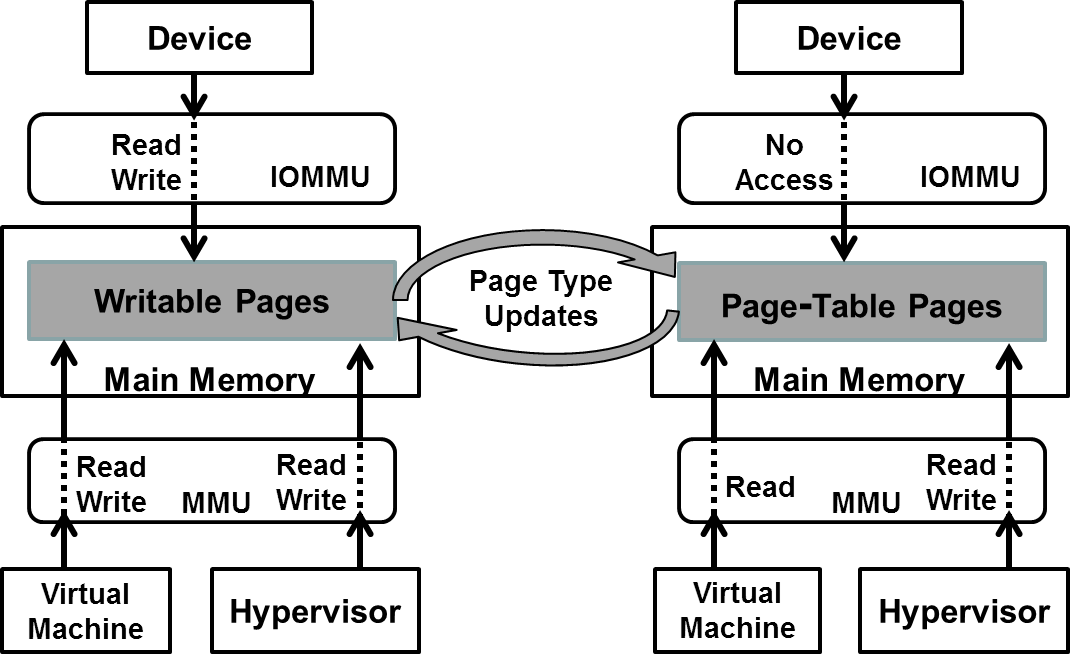
\includegraphics[width=0.5\textwidth]{image/background/wr2pt.png} \\
\caption{The page type updates between writable and page-table pages.}
\label{fig:wr2pt}
\end{figure}




Based on the observations, we are motivated to propose \name in order to reduce as many IOTLB flushes as possible for a maximum possible use of the IOTLB-path while retain the safety.
